\documentclass{article}
\usepackage{amsmath}
\usepackage{amssymb}
\usepackage{tikz}
\usetikzlibrary{arrows.meta, positioning}
\tikzset{%
    block/.style = {draw=black,rectangle,thick,
        minimum height=2em, text width=20em, align=center},
    line/.style = {draw=cyan, line width=3pt, 
        -{Triangle[length=6pt, width=8pt]}, shorten >=2pt, shorten <=2pt},
}


\begin{document}
{\large Continuum mechanics}
\vskip 0.2in
\noindent
In a flow problem on a 2D domain $\Omega$, the primary physical variable is the velocity field $u : \Omega \rightarrow \mathbb{R}^2$.
This field evolves in accord with continuum versions of Newton's laws of motion.
The Cauchy momentum equation is the $F = ma$ of continuum mechanics. It can be stated as an integral conservation law quantified
over all pieces of space, $\Omega_0 \subset \Omega$:
\begin{align*}
\frac{d}{dt} \int_{\Omega_0(t)} \rho u(\hat{x}) \,d\hat{x} &= \int_{\Omega_0}F(\hat{x})\,d\hat{x} + \oint_{\partial \Omega_0} \sigma(\hat{x})\cdot\hat{n}\,d\hat{x}.\\
\end{align*}
This says that the rate of change of total momentum (pointwise $\rho u$) in the piece $\Omega_0$, as it moves with the material,
is accounted for by body forces (pointwise $F$) and the \textit{tractions} (pointwise $\sigma\cdot\hat{n}$ on the boundary of the piece of space),
which measure internal forces due to the interaction of nearby material elements. $\sigma$, a $2\times 2$ matrix for each point in $\Omega$, is the \textit{Cauchy stress tensor}, and its specification
determines the properties of the material model. Conservation of mass is written as
\begin{align*}
\frac{d}{dt} \int_{\Omega_0(t)} \rho\,d\hat{x} = 0,
\end{align*}
which simply says that the piece $\Omega_0(t)$ has constant mass.


\vskip 0.2in
{\large The Stokes equations}
\vskip 0.2in
\noindent
The incompressible Navier-Stokes equations are formed by a Cauchy momentum equation ($F = ma$),
along with a stronger version of mass conservation, incompressibility (conservation of volume):
    $$\oint_{\partial\Omega_0}u\cdot\hat{n}\,d\hat{x} \text{\quad\quad for all pieces $\Omega_0 \in \Omega$}.$$
These equations model an incompressible Newtonian fluid
with traction forces $\sigma\cdot\hat{n}$ being decomposable into two parts:
\begin{itemize}
    \item A viscous force (which causes adjacent particles
in the fluid to tend to the same speed, like a ``velocity diffusion''),
    \item and an isotropic force which pushes
    small pieces of the material apart from eachother, in order for the flow to obey the incompressibility constraint.
\end{itemize}
This second force is due to the pressure field $p : \Omega \rightarrow \mathbb{R}$, which is a Lagrange multiplier
for the incompressibility constraint. The Navier-Stokes equations, in integral ``primal-dual'' form (solved for both
$u$ and the Lagrange multiplier $p$), are
\begin{align*}
\end{align*}

\vskip 0.2in
\begin{align*}
\int_{\Omega_0} \rho \frac{\partial u(\hat{x})}{\partial t}\,d\hat{x}
+ \oint_{\Omega_0}\rho u(u\cdot \hat{n})\,d\hat{x}
    \int_{\Omega_0}F(\hat{x})\,d\hat{x} + \oint_{\partial \Omega_0} \sigma(\hat{x})\cdot\hat{n}\,d\hat{x}.\\
\end{align*}


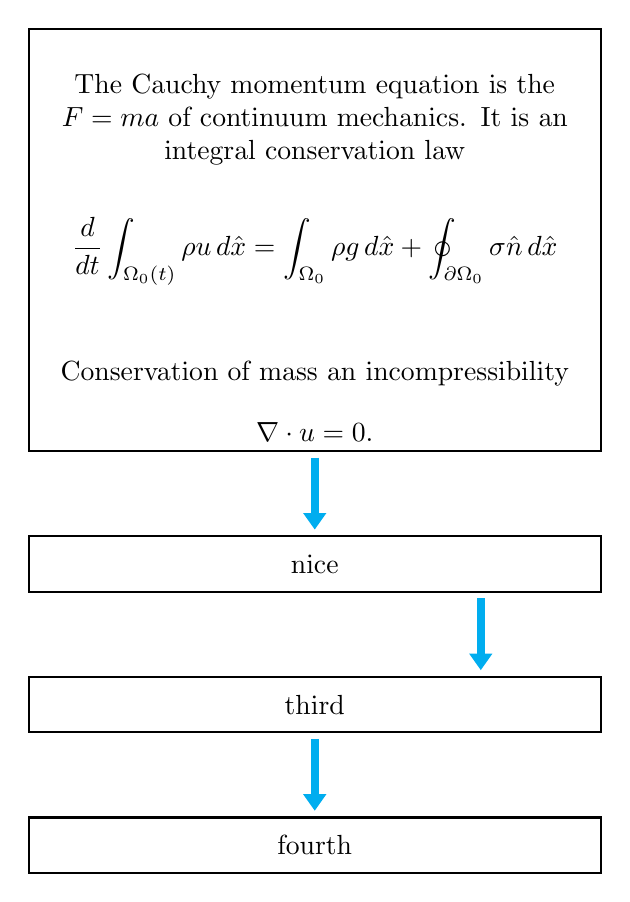
\begin{tikzpicture}[node distance = 2cm, auto] 
    \node [block] (init) {
\begin{center}
The Cauchy momentum equation is the $F = ma$ of continuum mechanics. It is an integral conservation law
\end{center}
\begin{align*}
\frac{d}{dt} \int_{\Omega_0(t)} \rho u \,d\hat{x} &= \int_{\Omega_0}\rho g\,d\hat{x} + \oint_{\partial \Omega_0} \sigma\hat{n}\,d\hat{x}\\
\end{align*}
\begin{center}
Conservation of mass an incompressibility
\begin{align*}
\nabla\cdot u = 0.
\end{align*}
\end{center}
}; 
    \node [block, below=30pt of init] (expert) {
nice}; 
    \path [line] (init) -- (expert); 
    \node [block, below=30pt of expert] (third) {third}; 
    \path [line] ([xshift=6em]expert.south) -- ([xshift=6em]third.north); 
    \node [block, below=30pt of third] (fourth) {fourth}; 
    \path [line] (third.south) -- (fourth.north); 
\end{tikzpicture}

\end{document}

